\subsection{Winston cones refurbishment}

Winston Cones (WC) are used to collect light onto the PMTs. In the LTCC there are three kind of WC:

\begin{enumerate}

\item Small
	\begin{enumerate}
		\item Height: 18cm
		\item Parallel Plate distance: 14cm
		\item Radius at the top: 20cm
		\item Radius at the bottom: 11cm
		\item Material: copper (electro-formed)
	\end{enumerate}

	\item Medium
	\begin{enumerate}
		\item Height: 22cm
		\item Parallel Plate distance: 15cm
		\item Radius at the top: 20cm
		\item Radius at the bottom: 11cm
		\item Material: 0.2” plastic (vacuum pressed)
	\end{enumerate}

	\item Large
	\begin{enumerate}
		\item Height: 30cm
		\item Parallel Plate distance: 18cm
		\item Radius at the top: 22cm
		\item Radius at the bottom: 11cm
		\item Material: copper (electro-formed)
	\end{enumerate}
\end{enumerate}

\begin{figure}
	\centering
	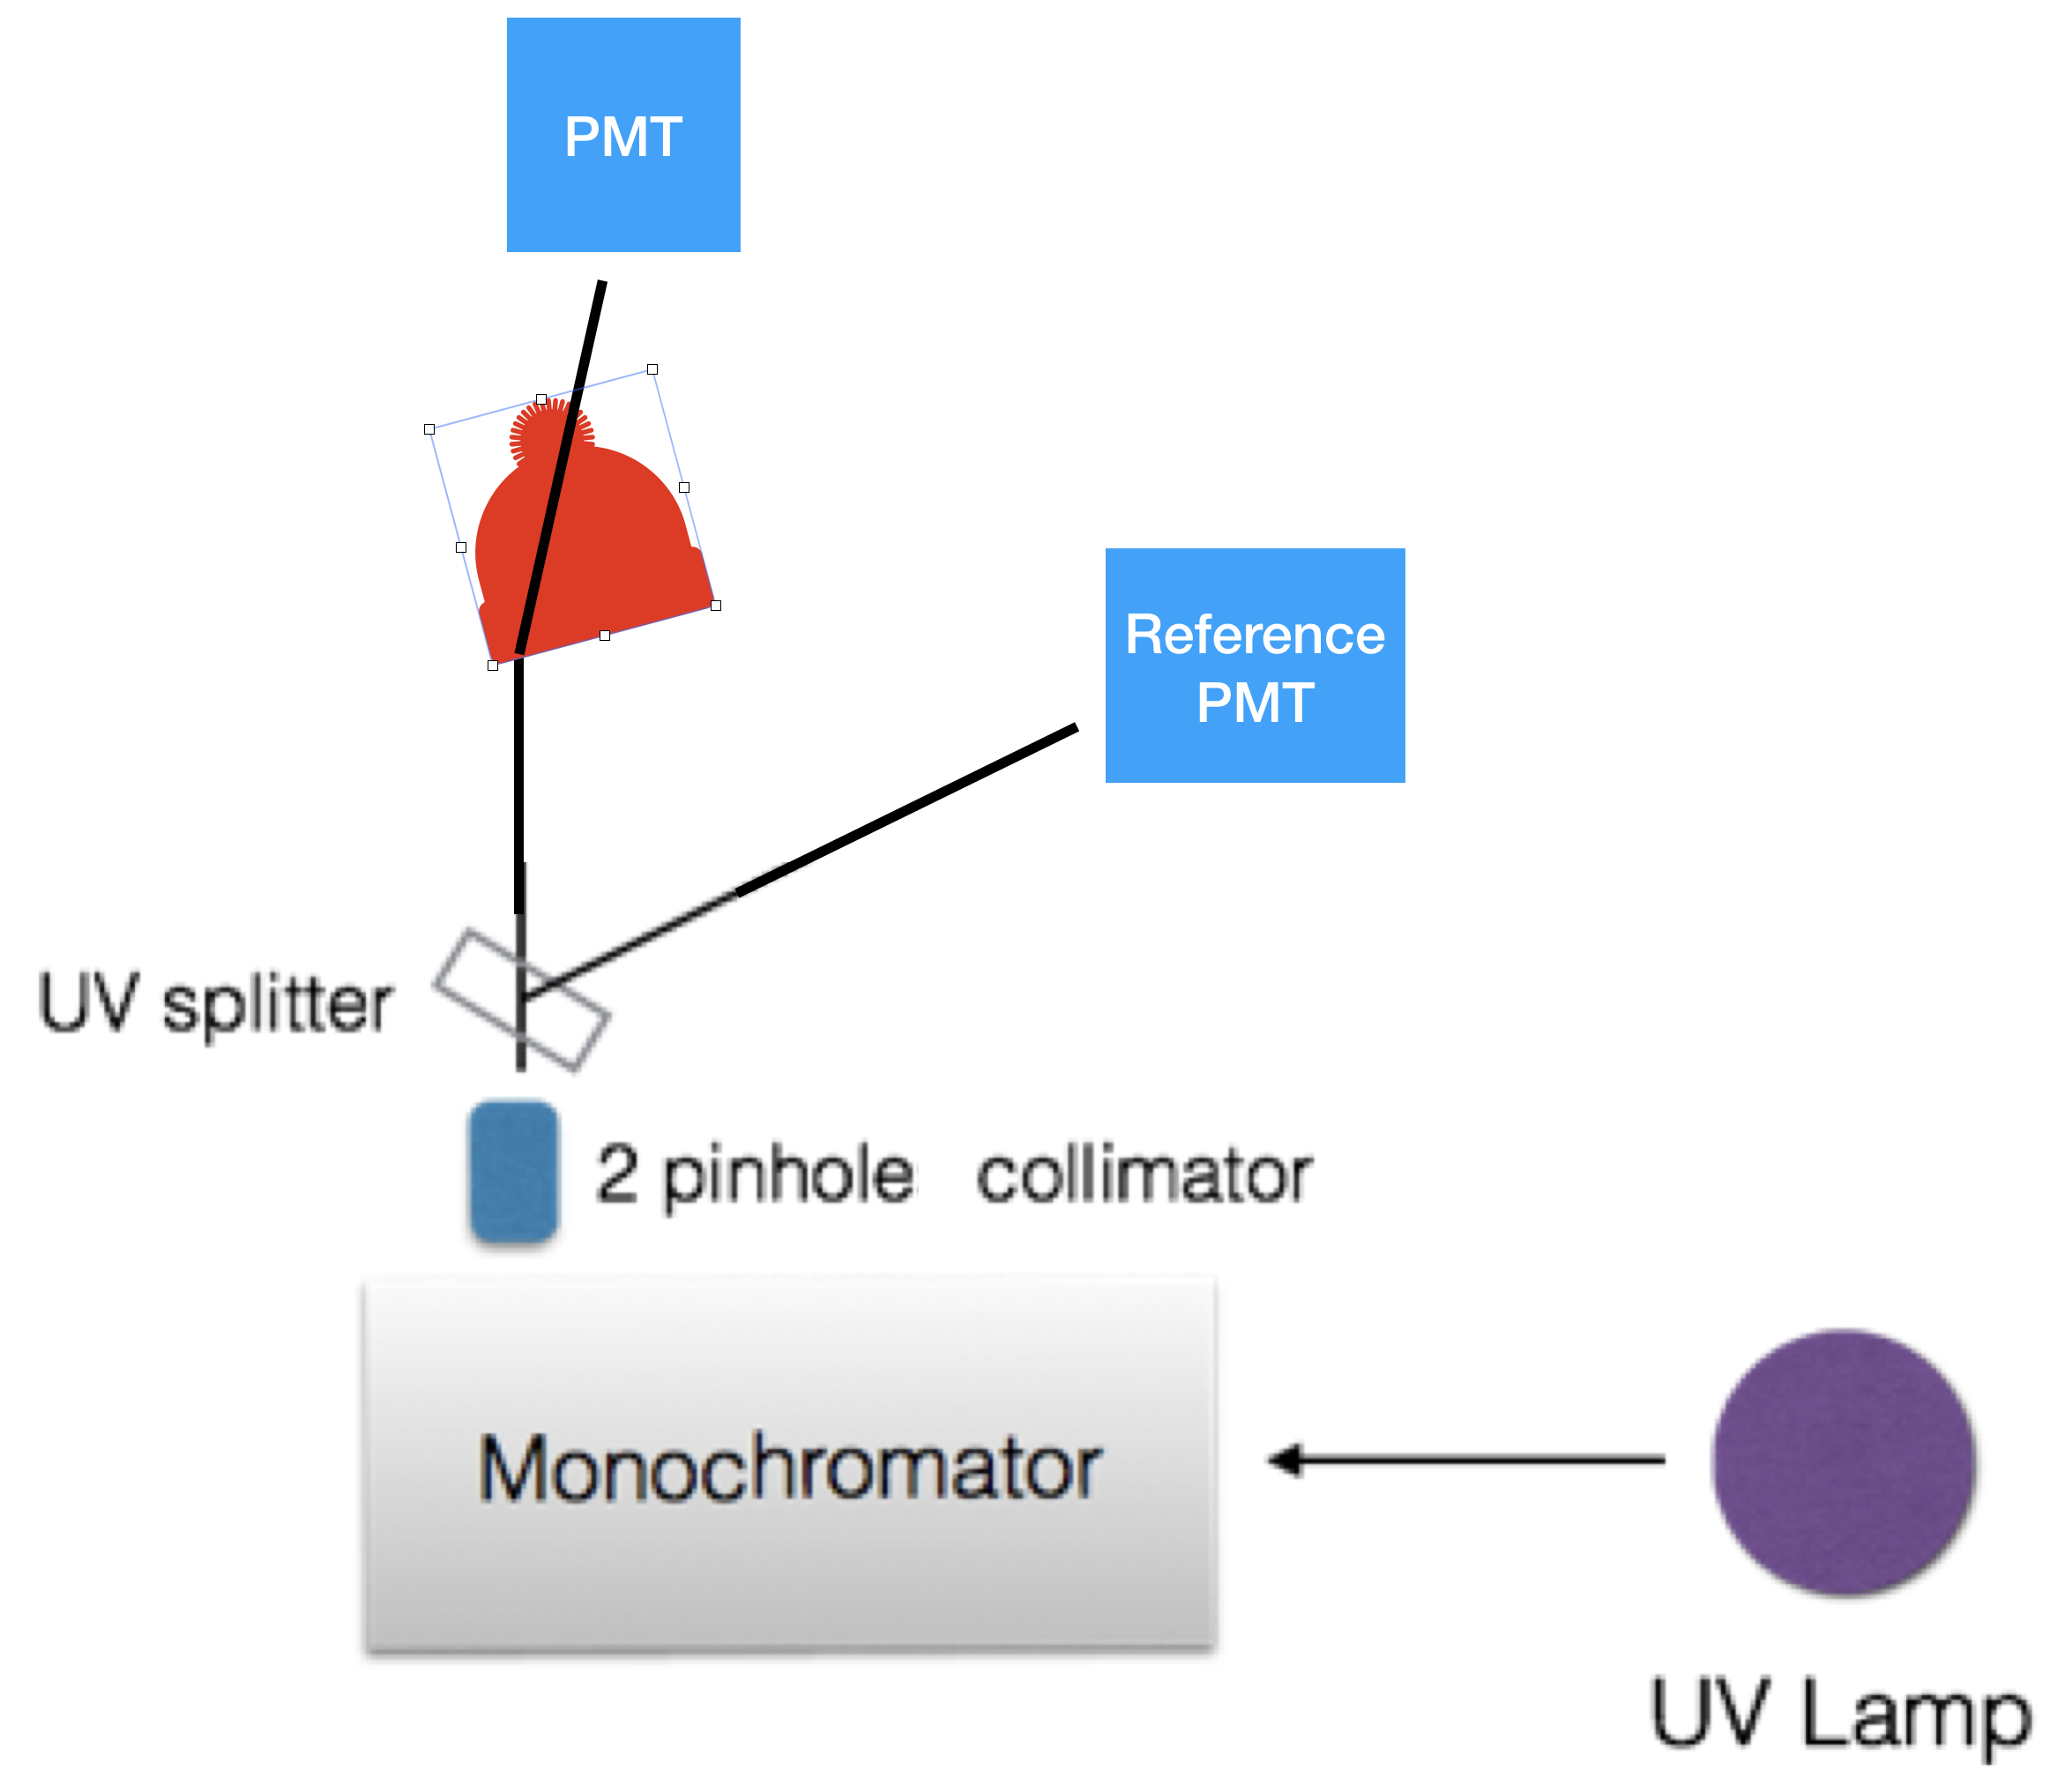
\includegraphics[width=0.95\columnwidth,keepaspectratio]{img/wcSetup.png}
	\caption{Setup to measure the WC reflectivity. The wavelength of light from a deuterium lamp was measured using a mono-chromator and splitted in two
            light beams, each with calibrated intensity. One of the light beam impinged on the WC at a typical angle of 12 degrees,
            while the other was directed at the reference PMT. }
	\label{fig:wcSetup}
\end{figure}

The reflectivity of the WC showed the same degradation as the mirrors. However due to their shape, re-coating of the WC is more costly than the mirrors and the budget allowed
to refurbish only 160 out of 216 total WCs.
A setup on an optical bench to measure the reflectivity for all the cones at wavelengths between 200 and 400 nm was designed to accept incident
shallow angles of 10-15 degrees (typical incident angle based on simulation studies), see \F{wcSetup}. A typical reflectivity of a poor WC is shown in \F{wcStatusBefore} (top).
All 216 WC were measured, and the results are shown in \F{wcStatusBefore} (top). This allowed to catalog the quality of the WC and to select the worse ones to refurbish,
see \F{wcStatusBefore} (bottom).
The cones were put in a vacuum chamber and $AlMg_2$ was deposited on top of the existing coating. A typical reflectivity of WC after a is shown in \F{wcStatusAfter} (top).
About 30 cones needed the additional treatment of removing the existing aluminum coating to improve the new $AlMg_2$ deposition. Even then, about half of these cones did not show improvements.
The results of the cones refurbishment are summarized in \F{wcStatusAfter} (bottom).


\begin{figure}
	\centering
	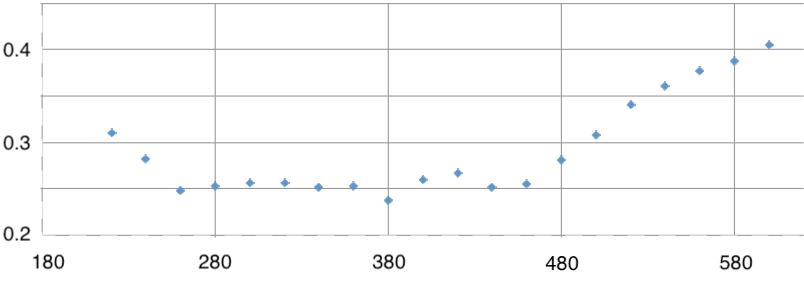
\includegraphics[width=0.95\columnwidth,keepaspectratio]{img/winstoConeSample2Reflectivity.png}
	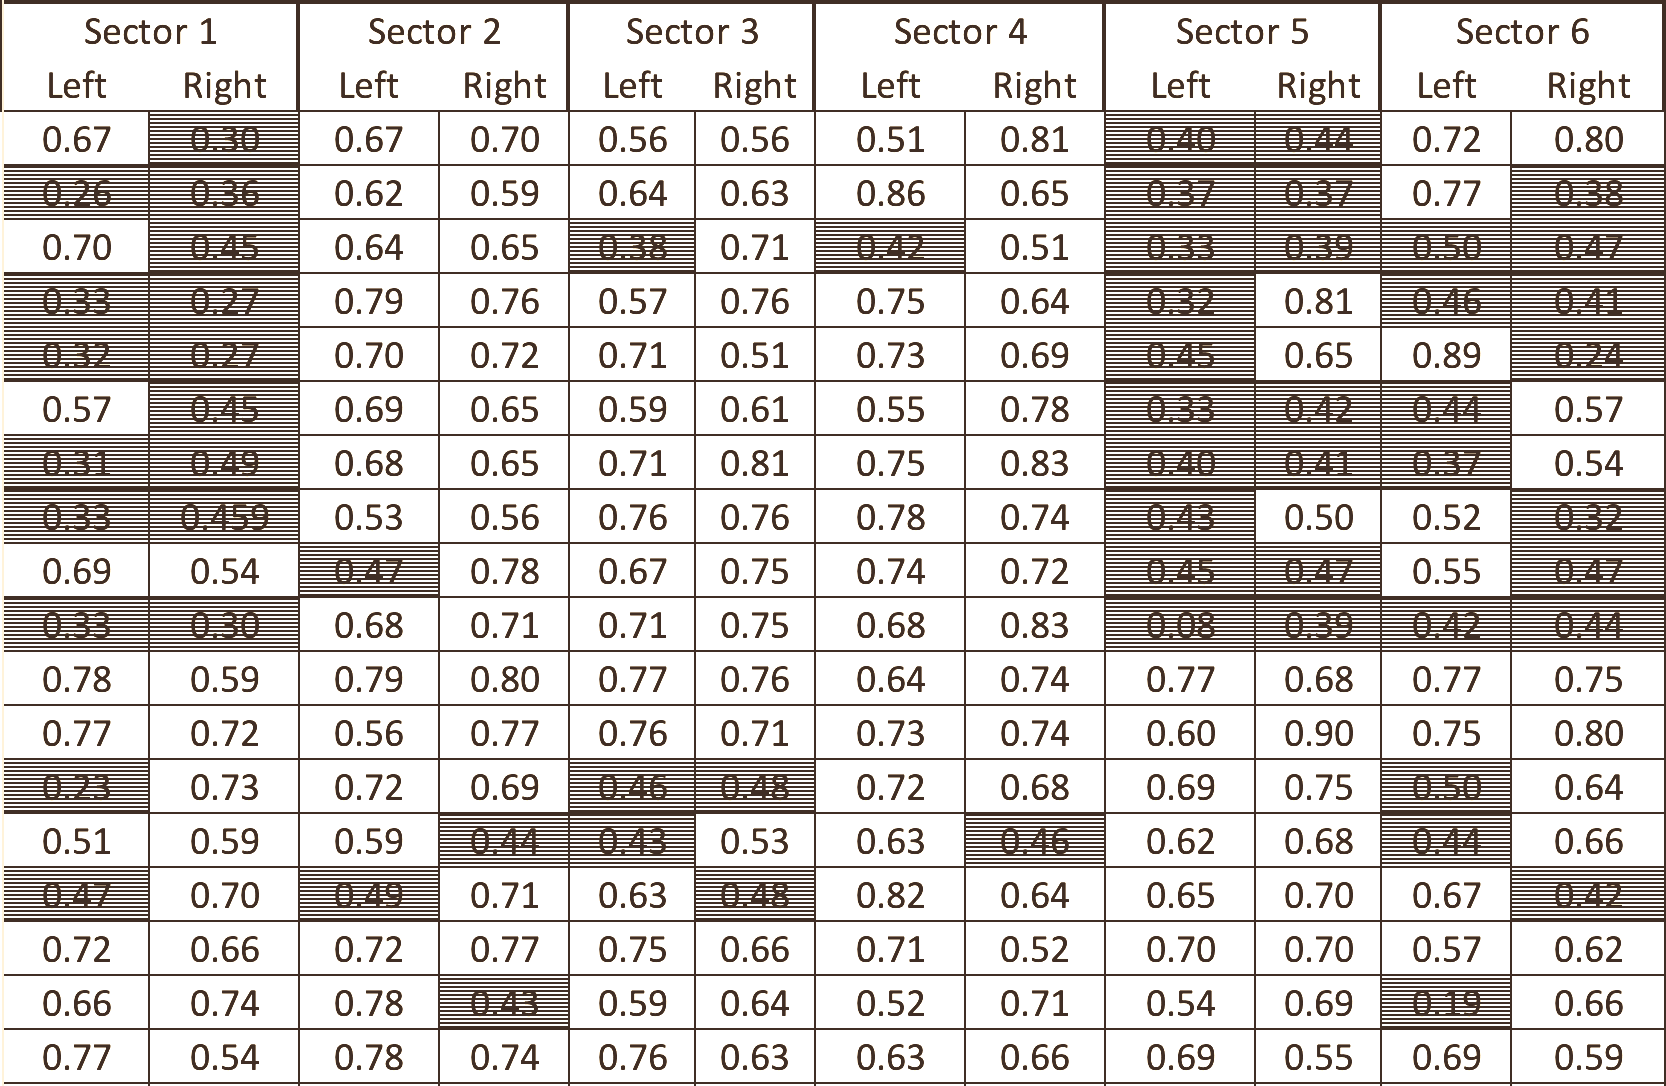
\includegraphics[width=0.95\columnwidth,keepaspectratio]{img/wcStatusBefore.png}
	\caption{Top: typical reflectivity of a "very poor" WC. The reflectivity is below 30\% for most of the wavelength between 200 and 400 nm. Bottom: the average reflectivity $r$ between 200 and 400 nm for
            all the WC. Legend: grey: ``very poor'' ($r < 30\%$); red: ``poor`` (30\% < $r < 50\%$); brown: ``so-so`` (50\% < $r < 70\%$); green: ``good`` (70\% < $r < 80\%$); yellow: ``excellent`` ( $r > 70\%$); }
	\label{fig:wcStatusBefore}
\end{figure}


\begin{figure}
	\centering
	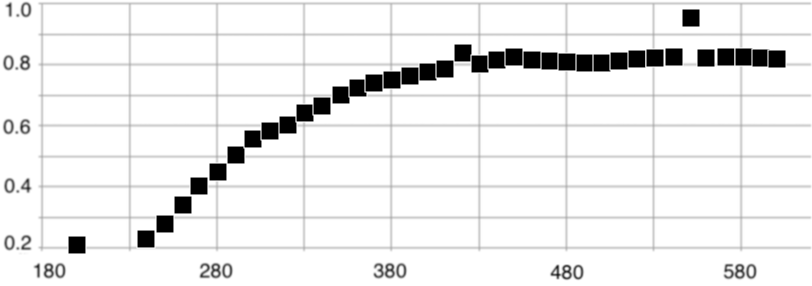
\includegraphics[width=1.0\columnwidth,keepaspectratio]{img/winstoConeSample1Reflectivity.png}
	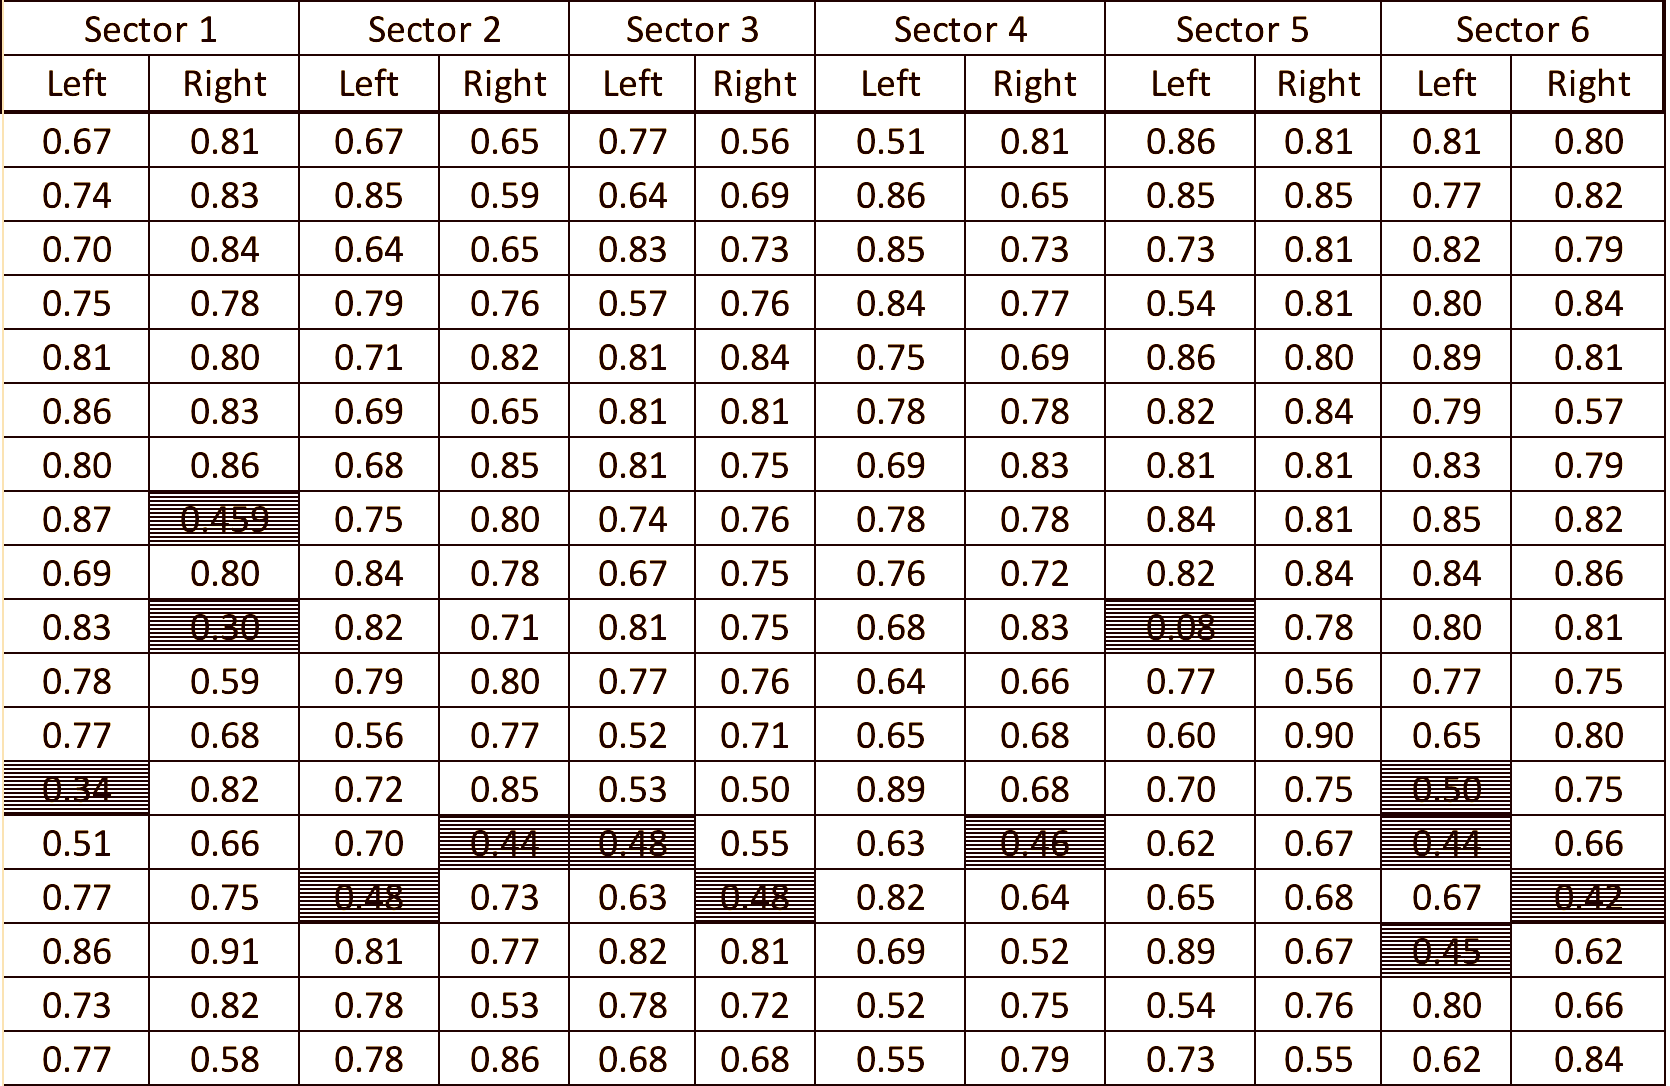
\includegraphics[width=1.0\columnwidth,keepaspectratio]{img/wcStatusAfter.png}
	\caption{Top: typical reflectivity of a "very poor" WC after refurbishment. The reflectivity quickly rise to $to\%$ at a wavelength of about 340 nm. Bottom: average WC reflectivity  $r$ between 200 and 400 nm for
				all the WC. This picture should be compared to \F{wcStatusAfter}. }
	\label{fig:wcStatusAfter}
\end{figure}


